% TikZ diagrams for the DREAM <-> n_TOF matching calibration.
% Defined as macros so the same source can be dropped into the slides and into
% any other document. Requires: tikz + libraries arrows, positioning,
% shapes.geometric, fit, backgrounds, calc (all present in TeX Live 2023 base).

\usetikzlibrary{arrows,positioning,shapes.geometric,fit,backgrounds,calc}

\definecolor{stagecol}{RGB}{31,90,150}
\definecolor{incol}{RGB}{110,110,110}
\definecolor{outcol}{RGB}{20,110,60}
\definecolor{ntofcol}{RGB}{225,238,250}
\definecolor{dreamcol}{RGB}{252,238,225}

\tikzset{
  stage/.style   = {rectangle, rounded corners=2pt, draw=stagecol, very thick,
                    fill=stagecol!8, align=center, inner sep=4pt,
                    text width=#1, font=\scriptsize},
  input/.style   = {align=center, font=\tiny\itshape, text=incol,
                    text width=2.55cm},
  deliver/.style = {rectangle, rounded corners=1pt, draw=outcol!60,
                    fill=outcol!7, align=center, font=\tiny, text=outcol!60!black,
                    inner sep=3pt, text width=2.55cm},
  flow/.style    = {-latex, very thick, draw=stagecol!70},
  thin flow/.style = {-latex, thick, draw=incol!70},
  grouplab/.style = {font=\scriptsize\bfseries, text=#1},
  box/.style     = {rectangle, rounded corners=2pt, draw=black!45, thick,
                    fill=black!3, align=center, inner sep=4pt,
                    text width=#1, font=\scriptsize},
}

% ------------------------------------------------------------------
% [1] The calibration chain: inside n_TOF first, then DREAM onto it.
% ------------------------------------------------------------------
\newcommand{\calibchaindiagram}{%
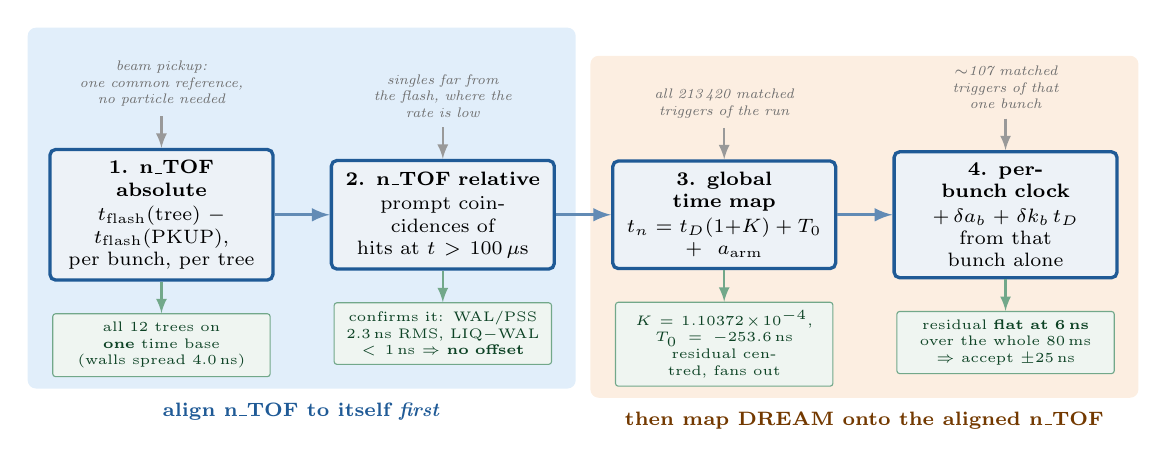
\begin{tikzpicture}[node distance=3.2mm]

  \node[stage=2.55cm] (s1)
       {\textbf{1. n\_TOF absolute}\\[1pt]
        $t_{\rm flash}({\rm tree})-t_{\rm flash}({\rm PKUP})$,\\ per bunch, per tree};
  \node[stage=2.55cm, right=7mm of s1] (s2)
       {\textbf{2. n\_TOF relative}\\[1pt]
        prompt coincidences of\\ hits at $t>100\,\mu$s};
  \node[stage=2.55cm, right=7mm of s2] (s3)
       {\textbf{3. global time map}\\[1pt]
        $t_{n}=t_{D}(1{+}K)+T_0$\\ $+\;a_{\rm arm}$};
  \node[stage=2.55cm, right=7mm of s3] (s4)
       {\textbf{4. per-bunch clock}\\[1pt]
        $+\,\delta a_b + \delta k_b\,t_{D}$\\ from that bunch alone};

  \foreach \a/\b in {s1/s2, s2/s3, s3/s4} \draw[flow] (\a) -- (\b);

  \node[input, above=4mm of s1] (i1) {beam pickup:\\ one common reference,\\ no particle needed};
  \node[input, above=4mm of s2] (i2) {singles far from\\ the flash, where the\\ rate is low};
  \node[input, above=4mm of s3] (i3) {all 213\,420 matched\\ triggers of the run};
  \node[input, above=4mm of s4] (i4) {$\sim$107 matched\\ triggers of that\\ one bunch};
  \foreach \a/\b in {i1/s1, i2/s2, i3/s3, i4/s4} \draw[thin flow] (\a) -- (\b);

  \node[deliver, below=4mm of s1] (o1)
       {all 12 trees on\\ \textbf{one} time base\\ (walls spread 4.0\,ns)};
  \node[deliver, below=4mm of s2] (o2)
       {confirms it: WAL/PSS\\ 2.3\,ns RMS, LIQ$-$WAL\\ $<1$\,ns $\Rightarrow$ \textbf{no offset}};
  \node[deliver, below=4mm of s3] (o3)
       {$K=1.10372\!\times\!10^{-4}$,\\ $T_0=-253.6$\,ns\\ residual centred, fans out};
  \node[deliver, below=4mm of s4] (o4)
       {residual \textbf{flat at 6\,ns}\\ over the whole 80\,ms\\ $\Rightarrow$ accept $\pm25$\,ns};
  \foreach \a/\b in {s1/o1, s2/o2, s3/o3, s4/o4} \draw[thin flow, draw=outcol!60] (\a) -- (\b);

  \begin{scope}[on background layer]
    \node[fit=(i1)(o2), rounded corners=3pt, fill=ntofcol, inner sep=3mm] (g1) {};
    \node[fit=(i3)(o4), rounded corners=3pt, fill=dreamcol, inner sep=3mm] (g2) {};
  \end{scope}
  \node[grouplab=stagecol, below=0.5mm of g1.south]
       {align n\_TOF to itself \emph{first}};
  \node[grouplab=orange!45!black, below=0.5mm of g2.south]
       {then map DREAM onto the aligned n\_TOF};
\end{tikzpicture}}

% ------------------------------------------------------------------
% [2] What is actually being matched, and how the fake rate is measured.
% ------------------------------------------------------------------
\newcommand{\matchflowdiagram}{%
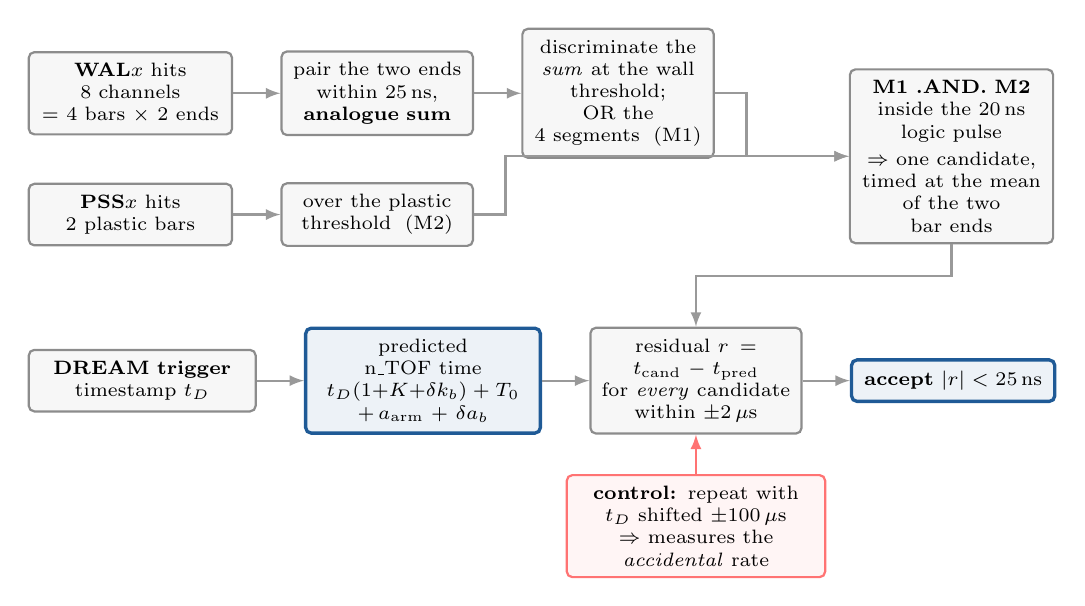
\begin{tikzpicture}[node distance=4mm]

  \node[box=2.3cm] (wal) {\textbf{WAL$x$} hits\\ 8 channels\\ $=$ 4 bars $\times$ 2 ends};
  \node[box=2.3cm, below=6mm of wal] (pss) {\textbf{PSS$x$} hits\\ 2 plastic bars};

  \node[box=2.15cm, right=6mm of wal] (sum)
       {pair the two ends\\ within 25\,ns,\\ \textbf{analogue sum}};
  \node[box=2.15cm, right=6mm of sum] (disc)
       {discriminate the\\ \emph{sum} at the wall\\ threshold; OR the\\ 4 segments \;(M1)};
  \node[box=2.15cm, right=6mm of pss] (pdisc)
       {over the plastic\\ threshold \;(M2)};

  \node[box=2.3cm, right=17mm of disc.east, yshift=-8mm] (and)
       {\textbf{M1 .AND. M2}\\ inside the 20\,ns\\ logic pulse\\[2pt]
        $\Rightarrow$ one candidate,\\ timed at the mean\\ of the two bar ends};

  \draw[thin flow] (wal) -- (sum);
  \draw[thin flow] (sum) -- (disc);
  \draw[thin flow] (pss) -- (pdisc);
  \draw[thin flow] (disc.east) -- ++(4mm,0) |- (and.west);
  \draw[thin flow] (pdisc.east) -- ++(4mm,0) |- (and.west);

  \node[box=2.6cm, below=13mm of pss.south west, anchor=north west] (dream)
       {\textbf{DREAM trigger}\\ timestamp $t_D$};
  \node[stage=2.7cm, right=6mm of dream] (map)
       {predicted n\_TOF time\\ $t_D(1{+}K{+}\delta k_b)+T_0$\\ $+\,a_{\rm arm}+\delta a_b$};
  \node[box=2.4cm, right=6mm of map] (res)
       {residual $r =$\\ $t_{\rm cand}-t_{\rm pred}$\\ for \emph{every} candidate\\ within $\pm2\,\mu$s};
  \node[stage=2.3cm, right=6mm of res] (win)
       {\textbf{accept} $|r|<25$\,ns};

  \draw[thin flow] (dream) -- (map);
  \draw[thin flow] (map) -- (res);
  \draw[thin flow] (res) -- (win);
  \draw[thin flow] (and.south) -- ++(0,-4mm) -| (res.north);

  \node[box=3.0cm, below=5mm of res.south, anchor=north, draw=red!55, fill=red!4]
       (ctl) {\textbf{control:} repeat with $t_D$ shifted $\pm100\,\mu$s\\
              $\Rightarrow$ measures the \emph{accidental} rate};
  \draw[thin flow, draw=red!55] (ctl) -- (res);
\end{tikzpicture}}
